\section{Secondary Groups}

%TODO: Explain format read from the Computer Vision group (and results if we manage to get some examples of their work), and output given to the Emotion Synthesis group
Our Secondary groups were Computer Vision (CV) and Emotion Synthesis (ES). Our task in the final pipeline was to read the input given by CV group and send the output to ES group.

\subsection{Computer Vision Group}
%Format read from CV Group
After training our models with the Bosphorus database we need to predict an emotion by reading input given from the CV group. They are giving input in a numpy array containing $25$ landmarks. PCA was used for dimensionality reduction before training our model, so the same PCA model is used on the given input for reducing the number of features. 

\subsection{Emotion Synthesis Group}
%Format given to Emotion Synthesis Group
We are using SVM model trained on Bosphorus Dataset as it is more stable and gives better accuracy as seen in the Implementation section. We are sending output in a JSON format which contatining all the six labels with their confidence score. Confidence scores tells us about the probability of the emotion predicted by our model. We are also sending a confusion matrix of our model so that they can get an idea of how well our model is performing for each of the labels.


\begin{figure}[H]
    \centering
    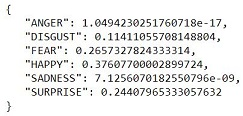
\includegraphics[height= 25mm]{figures/emotion_output.jpg}
    \caption{Output Format for ES Group}
    \label{emotion_output}
\end{figure}


%Reflection on how well the integration in the final pipeline worked
%what worked well
%what were challenges